\begin{frame}{Qu'est ce que la reproductibilité ?}

  \begin{block}{Définition}
    Une expérience est dite reproductible si elle peut être reproduite
    par son auteur ou un tiers de manière indépendante et arriver aux mêmes conclusions.
  \end{block}

  \begin{block}{Intérêt}
    \begin{itemize}
      \item Fondation de la méthode scientifique.
      \item Accélérateur de recherche: permet de construire sur des résultats établis.
      \item Visibilité: les résultats reproductibles sont plus cités
      \item Transparence: Résultats acceptés plus facilement
      \item Utile pour le transfert industriel
    \end{itemize}
  \end{block}

\end{frame}

\begin{frame}{Contexte \& État de l'art}

\begin{block}{Rapport de Collberg (2014)}
	\begin{itemize}
		\item 8 conférences ACM et 4 journaux.
		\item 102 résultats reproductibles sur 515 (80\% non-reproductible).
	\end{itemize}
\end{block}

	\begin{block}{Besoins}
  \begin{itemize}
  	\item Accès libre à la publication
  	\item Accès libre aux données
  	\item Accès libre aux composants logiciels utilisés
  	\item Environnement d'éxecution
  	\item Référence stables
  \end{itemize}
	\end{block}

\end{frame}

\begin{frame}{Niveaux de réalisme}
  \begin{block}{Simulation}
   Contrôle total des conditions
  \end{block}
  \begin{block}{Émulation}
    Prise en compte de l'architecture matérielle cible
  \end{block}
  \begin{block}{Plateforme de test}
   Passage à l'échelle
  \end{block}
  \begin{block}{Environnements réels}
    Conditions réelles
  \end{block}

  % \begin{figure}
  %   \centering
  %   \begin{tikzpicture}[->,>=latex,shorten >=1pt,auto,
  thick,main node/.style={fill=blue!20,draw}]

  \node[main node] (sim) {\begin{tabular}{c}Simulation\end{tabular}};
  \node[main node, right=of sim] (emu) {\begin{tabular}{c}Emulation\end{tabular}};
  \node[main node, right=of emu] (iotlab) {\begin{tabular}{c}Testbed\end{tabular}};
  \node[main node, right=of iotlab] (final) {\begin{tabular}{c}Déploiement\end{tabular}};

  \path
    (sim) edge[] (emu)
    % (emu) edge [bend left=10] node[below] {Modèle} (sim)

    (emu) edge[] (iotlab)
    % (iotlab) edge [bend left=10] node[below] {Prototype} (emu)

    (iotlab) edge[] (final)
    % (final) edge [bend left=10] node[below] {Finalisation} (iotlab)

;
\end{tikzpicture}
  % \end{figure}
  % \pnote{
  %   Simulateur: Controle total mais beaucoup de phénomènes sont modélisés
  % }
  % \pnote{
  %   Emulateur: Pareil que simulateur sauf qu'on développe pour une plateforme matérielle
  % }
  % \pnote{
  %   Testbed: Environnement relativement controlé et stable mais pas toujours représentatif
  % }
  % \pnote{
  %   Environnement réel: Réel mais de multiples pannes peuvent arriver.
  %   Logistique difficile.
  % }
\end{frame}

\begin{frame}\frametitle{Contexte \& État de l'art dans les réseaux de capteurs}

  \begin{block}{Contexte}
    \begin{itemize}
      \item Simulation (COOJA)
      \item Émulation de plateformes contraintes (MSPSIM)
      \item Déploiement sur des nœuds réels dans un banc de test (FIT IoT-lab)
    \end{itemize}
  \end{block}

  \begin{block}{État de l'art}
    \begin{itemize}
      \item Modélisation d'une expérience (Simulation)
      \item Fédérations de banc de test
      \item Difficile de passer d'une expérience sur simulation à un déploiement réel
    \end{itemize}
  \end{block}

  \pnote{
    - Les simulations ignorent beaucoup d'effets réels
    - L'émulation est un niveau plus proche du matériel Déploiement facile car on utilise le même binaire.
    - Les testbeds sont plus axés sur des déploiements concrets mais l'orchestration est difficile.
    - Conditions réelles => Tous les imprévus peuvent arriver.
  }

\end{frame}

\begin{frame}\frametitle{Enjeux de la recherche reproductible}

  \begin{block}{Recherche reproductible}
    \begin{itemize}
      \item Refaire une expérience.
      \item Partager facilement une expérience.
      \item Réduire le temps de mise en place d'une expérience.
    \end{itemize}
  \end{block}

  \pnote{Documente tous le process}
  \pnote{Facilite la mise en place de l'environnement}

\end{frame}

\begin{frame}\frametitle{Contribution}

  \begin{alertblock}{Makesense}
    \begin{itemize}
      \item Décompose une étape en une série d'étapes indépendantes les unes des autres.
      \item Permet d'avoir une exécution commune dans des contextes différents.
    \end{itemize}
  \end{alertblock}

  \begin{alertblock}{Outils}
    \begin{itemize}
      \item Notebook: Documentation \& Runtime.
      \item Moteur de gabarit.
      \item Gestion de version \& intégration continue.
    \end{itemize}
  \end{alertblock}

\end{frame}

\pnote{
  Évite de partager un seul gros script illisible et qui nécessite de
  faire une execution supplémentaire chaque fois que l'on change un paramètre.
}

\pnote{
  Evite par exemple d'avoir deux chemins d'executions séparés pour les cas de
  simulations et les cas de déploiements sur testbed.
}

\begin{frame}[shrink=5]\frametitle{Makesense Workflow}

  \begin{figure}[ht]
    \centering
    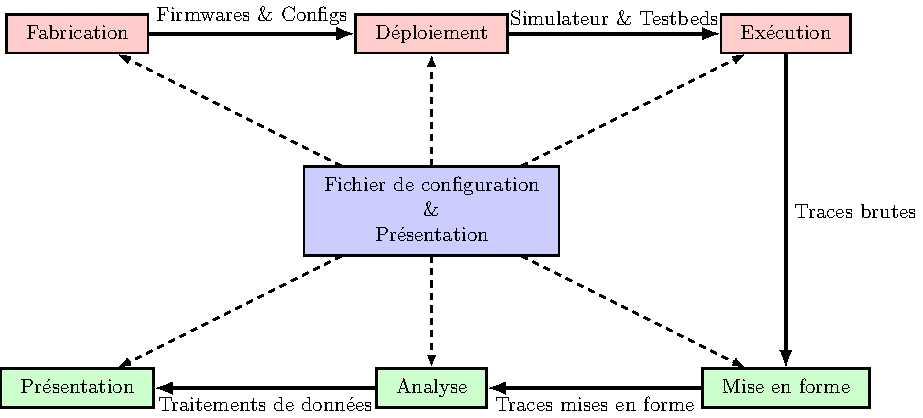
\includegraphics[scale=.75]{figures/makesense_workflow_slides.pdf}

  \end{figure}

  \pnote{
    - Insister sur l'idée de cycle et d'intégration continue.
  }
  \pnote{
    - Réduire le coût de tester une nouvelle idée en partant d'un déploiement réussi et en itérant par dessus.
  }

\end{frame}

\begin{frame}{Screenshot}
  \begin{figure}
    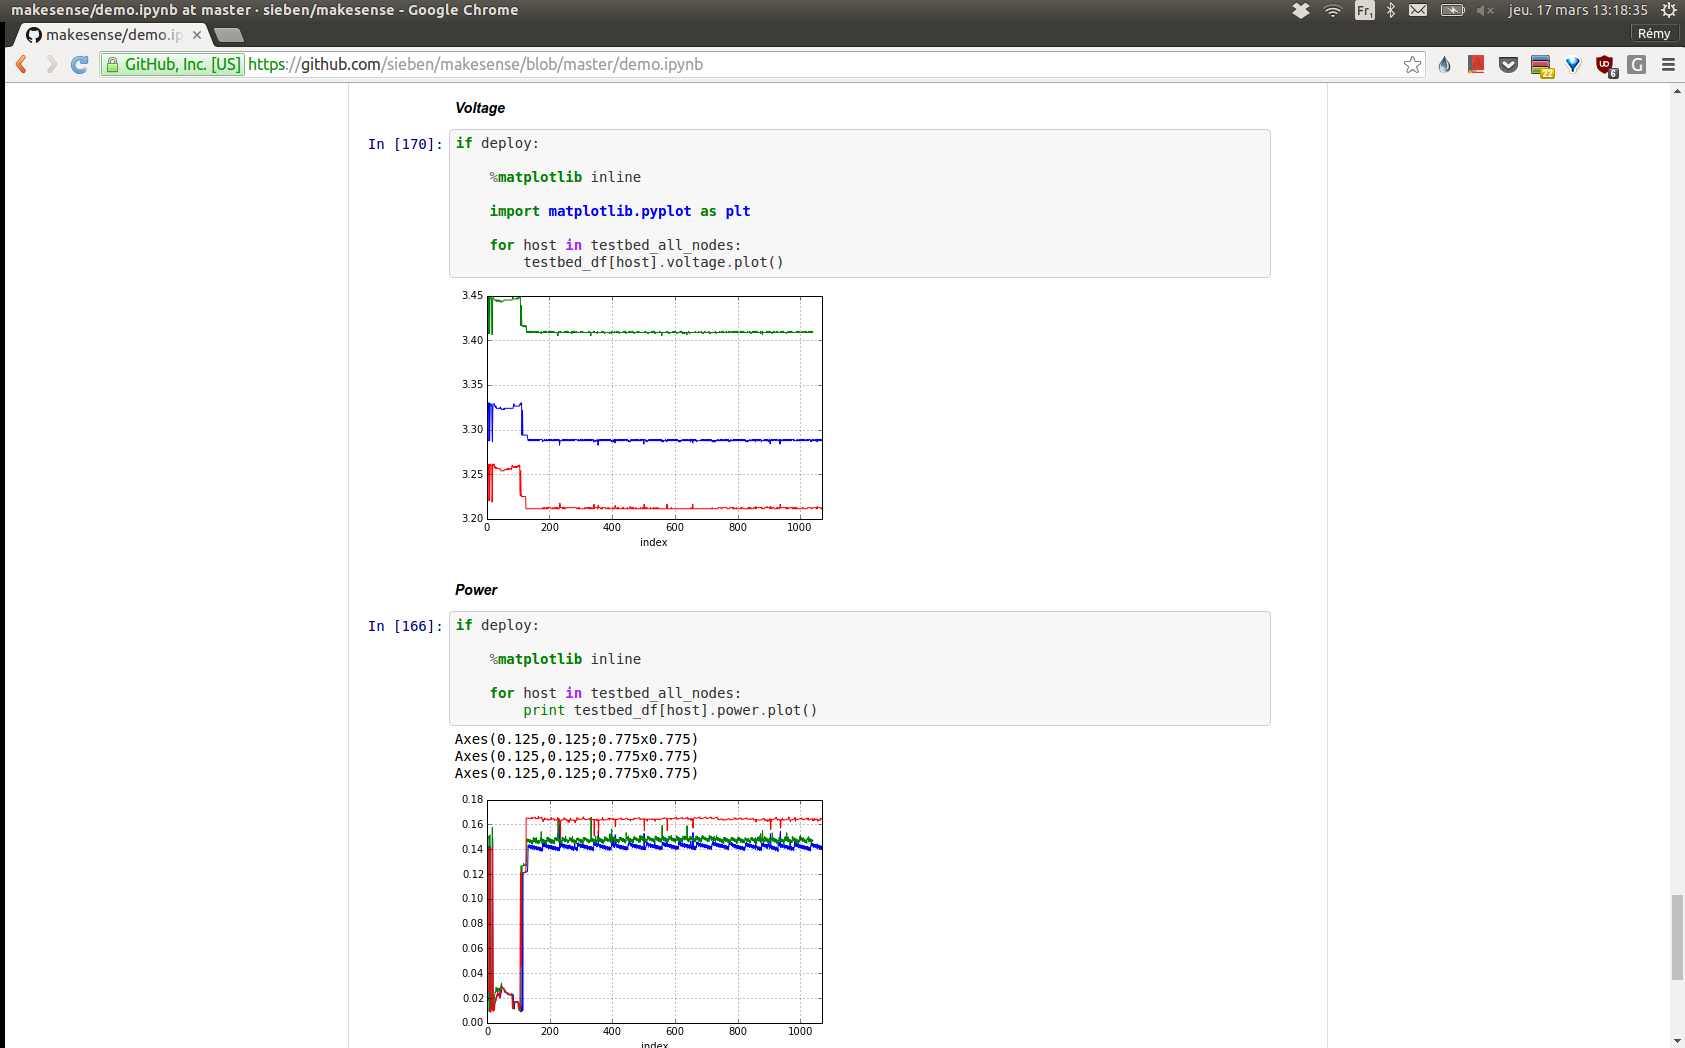
\includegraphics[width=\textwidth]{figures/jupyter_screenshot.png}
  \end{figure}
  \pnote{
    - Résultats pris sur IoT-lab Grenoble.
  }
  \pnote{
    - RPL UDP deux client et un serveur.
  }
\end{frame}

\begin{frame}{Gestion des traces}
  \begin{figure}
    \centering
    \begin{tikzpicture}[->,>=latex,shorten >=1pt, thick,main node/.style={fill=blue!20,draw}]

  \node[main node] (parse) {\begin{tabular}{c}Mise en forme\end{tabular}};

  \node[main node, below left=of parse] (pcap) {\begin{tabular}{c}PCAP\end{tabular}};
  \node[main node, above left=of parse] (logs) {\begin{tabular}{c}Logs\end{tabular}};

  \node[main node, right=of parse] (good_data) {\begin{tabular}{c}Données mises en forme\end{tabular}};
  \node[main node, above=of good_data] (analysis) {\begin{tabular}{c}Analyse des données\end{tabular}};

  \node[main node, below=of good_data] (csv) {\begin{tabular}{c}Export vers CSV\end{tabular}};

  \path
       (pcap) edge[->] (parse.south west) 
       (logs) edge[->] (parse.north west) 
       (parse) edge[->] (good_data) 
       (good_data)  edge[->] (analysis)
       (good_data) edge[->] (csv) 
  ;

\end{tikzpicture}

  \end{figure}

  \pnote{
    L'objectif de cette phase est de distinguer le décodage d'une information et son interprétation
  }
  \pnote{
    Le décodage ça transforme des données inintelligibles (binaires) vers du texte
  }
  \pnote{
    L'interprétation se base sur des quantités qualitatives ou quantitatives pour donner une conclusion
  }
\end{frame}

% \begin{frame}
%   TODO: Mettre autant de captures d'écran que possibles
% \end{frame}

\begin{frame}\frametitle{Conclusion}

  \begin{alertblock}{Makesense}
    \begin{itemize}
      \item Réduction du temps de démarrage
      \item Réduire le temps nécessaire pour migrer une simulation vers un testbed
      \item Eviter le Not Invented Here
      \item Le notebook est une bonne interface pour présenter des résultats
    \end{itemize}
  \end{alertblock}

  \begin{alertblock}{Recherche Reproductible}
  \begin{itemize}
    \item Nécessité de la méthode scientifique
    \item Des outils existent pour la rendre accessible.
  \end{itemize}
  \end{alertblock}

  \pnote{
    - L'objectif est de réduire le cout de la mise en place et du partage.
  }
  \pnote{
    - Mentionner qu'il faut qu'elle devienne un critère pour les publications autrement elle ne sera pas appliquée.
  }
  \pnote{
    - Pas de mesures de download sur github (Tache difficile)
  }
  \pnote{
    - Notebook utilisé largement: Makesense est une application de ce concept.
  }
\end{frame}

% \begin{frame}
%     \item R{\'e}my Leone, Jeremie Leguay, Paolo Medagliani, Claude Chaudet, et~al.
% \newblock Makesense: Managing reproducible wsns experiments.
% \newblock {\em Fifth Workshop on Real-World Wireless Sensor Networks}, 2013.

%   \item R{\'e}my L{\'e}one, J{\'e}r{\'e}mie Leguay, Paolo Medagliani, and Claude
%   Chaudet.
% \newblock Demo abstract: Makesense—managing reproducible wsns experiments.
% \newblock In {\em Real-World Wireless Sensor Networks}, pages 65--71. Springer,
%   2014.

%   \item R{\'e}my L{\'e}one, J{\'e}r{\'e}mie Leguay, Paolo Medagliani, and Claude
%   Chaudet.
% \newblock Demo Abstract: Automating WSN experiments and simulations.
% \newblock In {\em EWSN}, 2015.

%  \item Invitation au colloque R4: Retour d'expéRiences sur la Recherche Reproductible.
%   \newblock Le Studium - Centre International Universitaire pour la Recherche - Orléans
%   \newblock 3 et 4 Décembre 2015

% \end{frame}


  % \begin{alertblock}{Évolution de la méthodologie de recherche reproductible}
  %     \begin{itemize}
  %       \item Nombre d'utilisateurs/d'implémentations en augmentation
  %       \item Le matériel via les testbeds facilite l'accès
  %       \item La difficulté vient de l'intégration et du passage à l'échelle
  %       \item Support interactifs, testés et à jour
  %     \end{itemize}
  % \end{alertblock}
